\section{Introduction}
\IEEEPARstart{I}{ndustrial} agents can propose process changes, but a runtime must resolve the production context and map each proposal to the intended control signal before dispatch. That mapping depends on the scene. On a cast-film line, for example, a line-speed setpoint may affect film thickness, yet the setpoint and thickness measurement remain distinct variables even when both use Message Queuing Telemetry Transport (MQTT). A service receipt, a device readback, and a later process measurement also record different events. Fig.~\ref{fig:control-path} illustrates these distinctions.

Prior work addresses industrial-agent planning and control, programmable logic controller (PLC) program generation, protocol access, semantic commissioning, and plant-facing verification. Because these studies use different tasks and evaluation settings, their results are not directly comparable. This paper examines a narrower question: how should a runtime carry production context and signal meaning from a task-level proposal to device dispatch, while checking route-specific authority and limits? We do not propose a new planning policy or control law.

We implement this path in a configuration-driven runtime. Each scene binds its line, product, recipe, and run to separate acquisition and control nodes, registered drivers, process objectives, and write limits. Task-mediated and direct calls share a dispatcher, after which the selected handler resolves current state and applies its route-specific checks. Approval paths then revalidate the state relevant to that operation: recipe operations check the active context, while single-node writes check their binding and any applicable grant before the common controller checks the value. These checks reduce exposure to stale state, but they do not make authorization and device I/O atomic.

The contributions are:
\begin{enumerate}
  \item A production-scene configuration model that links operational context and direction-specific signal mappings to registered drivers, objectives, and limits at the operation boundary (Section~III).
  \item An implemented task-to-device path for registered agent harnesses and direct callers. It combines shared dispatch, route-specific checks, conditional approval, and common write guards, while retaining command outcomes, optional readbacks, and later process observations as separate records (Sections~III--V).
  \item An evidence-bounded evaluation of configured mappings and pre-dispatch guards across four simulated scenes, with command readback, process observations, and live-Agent outcomes reported separately (Section~VI).
\end{enumerate}

Section~II reviews industrial-agent, interface, and operation-governance work. Sections~III--V describe the runtime configuration, operation path, and write controls. Section~VI reports the evaluation by evidence type, and Section~VII discusses the limits of the results.

\begin{figure}[!b]
\centering
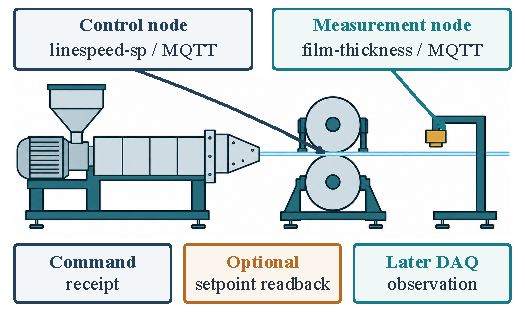
\includegraphics[width=0.98\columnwidth]{../figures/fig1.pdf}
\caption{Running cast-film example. MQTT maps the line-speed setpoint to a control node and film thickness to a separate measurement node. A command receipt, optional device readback, and later DAQ observation are distinct evidence; the illustration does not establish a causal process effect.}
\label{fig:control-path}
\end{figure}
